
%%%%%%%%%%%%%%%%%%%%%%%
% SN candidates table %
%%%%%%%%%%%%%%%%%%%%%%%

\begin{table}[p]
\caption{\label{tab:sn} Candidates classified as supernovae}
\begin{center}
\begin{footnotesizetabular}{lccccccc}

\hline
\hline
ID & Nickname & R.A. (J2000) & Decl. (J2000) & $z$ & Type & Conf. & How? \\
\hline
\multicolumn{8}{l}{\emph{Cluster Members}} \\
SCP06C1 & Midge & $12^{\rm h}\,29^{\rm m}\,33^{\rm s}.012$ & $+01^{\circ}\,51'\,36''.67$ & 0.98\phn & Ia & secure & a,c\\
SCP05D0 & Frida & $02^{\rm h}\,21^{\rm m}\,42^{\rm s}.066$ & $-03^{\circ}\,21'\,53''.12$ & 1.014 & Ia & secure & a,b,c\\
SCP06F12 & Caleb & $14^{\rm h}\,32^{\rm m}\,28^{\rm s}.748$ & $+33^{\circ}\,32'\,10''.05$ & 1.11\phn & Ia & probable & c\\
SCP06H5 & Emma & $14^{\rm h}\,34^{\rm m}\,30^{\rm s}.139$ & $+34^{\circ}\,26'\,57''.29$ & 1.231 & Ia & secure & b,c\\
SCP06K18 & Alexander & $14^{\rm h}\,38^{\rm m}\,10^{\rm s}.663$ & $+34^{\circ}\,12'\,47''.19$ & 1.412 & Ia & probable & b\\
SCP06K0 & Tomo & $14^{\rm h}\,38^{\rm m}\,08^{\rm s}.366$ & $+34^{\circ}\,14'\,18''.08$ & 1.416 & Ia & secure & b,c\\
SCP06R12 & Jennie & $02^{\rm h}\,23^{\rm m}\,00^{\rm s}.082$ & $-04^{\circ}\,36'\,03''.04$ & 1.212 & Ia & secure & b,c\\
SCP06U4 & Julia & $23^{\rm h}\,45^{\rm m}\,29^{\rm s}.429$ & $-36^{\circ}\,32'\,45''.73$ & 1.05\phn & Ia & secure & a,c\\
\multicolumn{8}{l}{\emph{Cluster Membership Uncertain}} \\
SCP06E12 & Ashley & $14^{\rm h}\,15^{\rm m}\,08^{\rm s}.141$ & $+36^{\circ}\,12'\,42''.94$ & \nodata & Ia & plausible & c\\
SCP06N32 & \nodata & $02^{\rm h}\,20^{\rm m}\,52^{\rm s}.368$ & $-03^{\circ}\,34'\,13''.32$ & \nodata & CC & plausible & c\\
\multicolumn{8}{l}{\emph{Not Cluster Members}} \\
SCP06A4 & Aki & $22^{\rm h}\,16^{\rm m}\,01^{\rm s}.077$ & $-17^{\circ}\,37'\,22''.09$ & 1.193 & Ia & probable & c\\
SCP06B3 & Isabella & $22^{\rm h}\,05^{\rm m}\,50^{\rm s}.402$ & $-01^{\circ}\,59'\,13''.34$ & 0.743 & CC & probable & c\\
SCP06C0 & Noa & $12^{\rm h}\,29^{\rm m}\,25^{\rm s}.654$ & $+01^{\circ}\,50'\,56''.58$ & 1.092 & Ia & secure & b,c\\
SCP06C7 & \nodata & $12^{\rm h}\,29^{\rm m}\,36^{\rm s}.517$ & $+01^{\circ}\,52'\,31''.47$ & 0.61\phn & CC & probable & c\\
SCP05D6 & Maggie & $02^{\rm h}\,21^{\rm m}\,46^{\rm s}.484$ & $-03^{\circ}\,22'\,56''.18$ & 1.314 & Ia & secure & b,c\\
SCP06F6 & \nodata & $14^{\rm h}\,32^{\rm m}\,27^{\rm s}.394$ & $+33^{\circ}\,32'\,24''.83$ & 1.189 & non-Ia & secure & a\\
SCP06F8 & Ayako & $14^{\rm h}\,32^{\rm m}\,24^{\rm s}.525$ & $+33^{\circ}\,33'\,50''.75$ & 0.789 & CC & probable & c\\
SCP06G3 & Brian & $14^{\rm h}\,29^{\rm m}\,28^{\rm s}.430$ & $+34^{\circ}\,37'\,23''.13$ & 0.962 & Ia & plausible & c\\
SCP06G4 & Shaya & $14^{\rm h}\,29^{\rm m}\,18^{\rm s}.743$ & $+34^{\circ}\,38'\,37''.38$ & 1.35\phn & Ia & secure & a,b,c\\
SCP06H3 & Elizabeth & $14^{\rm h}\,34^{\rm m}\,28^{\rm s}.879$ & $+34^{\circ}\,27'\,26''.61$ & 0.85\phn & Ia & secure & a,c\\
SCP06L21 & \nodata & $14^{\rm h}\,33^{\rm m}\,58^{\rm s}.990$ & $+33^{\circ}\,25'\,04''.21$ & \nodata & CC & plausible & c\\
SCP06M50 & \nodata & $16^{\rm h}\,04^{\rm m}\,25^{\rm s}.300$ & $+43^{\circ}\,04'\,51''.85$ & \nodata & \nodata & \nodata & \nodata\\
SCP05N10 & Tobias & $02^{\rm h}\,20^{\rm m}\,52^{\rm s}.878$ & $-03^{\circ}\,33'\,40''.20$ & 0.203 & CC & plausible & c\\
SCP06N33 & Naima & $02^{\rm h}\,20^{\rm m}\,57^{\rm s}.699$ & $-03^{\circ}\,33'\,23''.97$ & 1.188 & Ia & probable & c\\
SCP05P1 & Gabe & $03^{\rm h}\,37^{\rm m}\,50^{\rm s}.352$ & $-28^{\circ}\,43'\,02''.66$ & 0.926 & Ia & probable & c\\
SCP05P9 & Lauren & $03^{\rm h}\,37^{\rm m}\,44^{\rm s}.512$ & $-28^{\circ}\,43'\,54''.58$ & 0.821 & Ia & secure & a,c\\
SCP06U7 & Ingvar & $23^{\rm h}\,45^{\rm m}\,33^{\rm s}.867$ & $-36^{\circ}\,32'\,43''.48$ & 0.892 & CC & probable & c\\
SCP06X26 & Joe & $09^{\rm h}\,10^{\rm m}\,37^{\rm s}.889$ & $+54^{\circ}\,22'\,29''.07$ & 1.44\phn & Ia & plausible & c\\
SCP06Z5 & Adrian & $22^{\rm h}\,35^{\rm m}\,24^{\rm s}.966$ & $-25^{\circ}\,57'\,09''.61$ & 0.623 & Ia & secure & a,c \\
\hline
\end{footnotesizetabular}

\end{center}
{\footnotesize {\bf Note.} --- ``How?'' indicates how the type is
  determined.  (a) Spectroscopic confirmation.  (b) Host is
  morphologically early-type, with no signs of recent star formation.
  (c) Light curve shape, color, magnitude consistent with type. We do
  not assign a type for SCP06M50 because there is significant
  uncertainty that the candidate is a SN at all.}
\end{table}

After removing 17 image artifacts and 14 AGN, 29 candidates remain
(listed in Table~\ref{tab:sn}). One of these is the peculiar
transient SN~SCP06F6 which, as noted above, is clearly not a SN~Ia.
Note that Table~\ref{tab:sn} contains 10 fewer candidates than the
list presented by \citet{dawson09a}. This is unsurprising; here we have
intentionally used a stricter selection than in the original search,
the source for the \citet{dawson09a} sample. Still, after finalizing our
selection method we checked that there were no unexpected
discrepancies. Five of the \citet{dawson09a} candidates (SCP06B4, SCP06U2,
SCP06X18, SCP06Q31, SCP06T1) fell just below either the detection or
signal-to-noise thresholds in our selection. These were found in the
original search because detection thresholds were set slightly lower,
and because the images were sometimes searched in several different
ways. For example, in the original search SCP06B4 was only found by
searching an $i_{775}$ subtraction. Two \citet{dawson09a} candidates (SCP05D55,
SCP06Z52) were found too far on the decline and failed the light curve
requirements (\S\ref{sec:cands_lccuts}). Three \citet{dawson09a} candidates (SCP06X27,
SCP06Z13, SCP06Z53) were found while searching in ``follow-up''
visits, which were not searched here. SCP06U6 passed all requirements,
but is classified here as an AGN, as noted above. With the exception
of SCP06U6, all of these candidates are likely to be supernovae
(mostly core collapse). However, the types of candidates that did not
pass our requirements are not of concern for this analysis. Finally,
SCP06M50 was not reported in \citet{dawson09a}, but is classified here as a SN,
although with great uncertainty (discussed in detail
in \S\ref{sec:cands_sncomments}).

Thanks to the extensive ground-based spectroscopic follow-up campaign,
we were able to obtain spectroscopic redshifts for 25 of the 29
SNe. The redshift reported in Table~\ref{tab:sn} is derived from the
SN host galaxy for all but one candidate (SCP06C1) where the redshift
is from the SN spectrum itself. Of the 25 candidates with redshifts,
eight are in clusters and 17 are in the field. Note that this high
spectroscopic completeness is particularly important for determining
the cluster or non-cluster status of each SN, which directly affects
the determination of the cluster SN~Ia rate. The possible cluster
memberships of the four candidates lacking redshifts are discussed
below.

We determine the type of each of the 29 supernovae using a combination
of methods in order to take into account all available information for
each supernova. This includes (a) spectroscopic confirmation, (b) the
host galaxy environment, and (c) the SN light curve. To qualify the
confidence of each supernova's type, we rank the type as ``secure,''
``probable,'' or ``plausible'':
\begin{description}
\item[Secure SN~Ia] Has
spectroscopic confirmation or \emph{both} of the following: (1) an
early-type host galaxy with no recent star formation and (2) a light
curve with shape, color and magnitude consistent with SNe~Ia and
inconsistent with other types.
\item[Probable SN~Ia] Fulfills either the host galaxy 
requirement or the light curve requirement, but not both.
\item[Plausible SN~Ia] The light curve is indicative of a SN~Ia, 
but there is not enough data to rule out other types.
\item[Secure SN~CC] Has spectroscopic confirmation (note that 
there are no such candidates in this sample). 
\item[Probable SN~CC] The light curve is consistent with a 
core-collapse SN and inconsistent with a SN~Ia. 
\item[Plausible SN~CC] Has a light curve indicative
of a core-collapse SN, but not inconsistent with a SN~Ia. 
\end{description}
This ranking system is largely comparable to the ``gold,'' ``silver,''
``bronze'' ranking system of \citet{strolger04a}, except that we do
not use their ``UV deficit'' criterion. This is because our data do
not include the bluer F606W filter, and because SNe~Ia and CC are
only distinct in UV flux for a relatively small window early in the
light curve. Below, we discuss in detail the three typing methods used.

%Obtaining spectroscopic
%confirmation of SNe at $z \gtrsim 1$ remains notoriously difficult,
%whether from the ground or from space. In a high-redshift SN rate
%study, one cannot hope to obtain a spectroscopic type for \emph{every}
%SN candidate. Therefore, we rely on the properties of the host galaxy
%and the light curve of the SN in typing the majority of the
%supernovae.

{\bf (a) Spectroscopic confirmation:} During the survey, seven
candidates were spectroscopically confirmed as
SNe~Ia \citep{dawson09a,morokuma10a}. These seven (three of which are in
clusters) are designated with an ``a'' in the ``typing'' column of
Table~\ref{tab:sn}. All seven candidates have a light curve shape,
absolute magnitude and color consistent with a SN~Ia. Although the
spectroscopic typing by itself has some degree of uncertainty, the
corroborating evidence from the light curve makes these ``secure''
SNe~Ia.

{\bf (b) Early-type host galaxy:} The progenitors of core-collapse SNe
are massive stars ($> 8 M_{\odot}$) with main sequence lifetimes of
$<40$~Myr. Thus, core-collapse SNe only occur in galaxies with recent
star formation. Early-type galaxies, having typically long ceased star
formation, overwhelmingly host Type~Ia
SNe \citep[e.g.,][]{cappellaro99a,hamuy00a}. In fact, in an extensive
literature survey of core-collapse SNe reported in early-type
hosts, \citet{hakobyan08a} found that only three core-collapse SNe
have been recorded in early-type hosts, and that the three host
galaxies in question had either undergone a recent merger or were
actively interacting. In all three cases there are independent
indicators of recent star formation. Therefore, in the cases where the
host galaxy morphology, photometric color, and spectrum all indicate
an early-type galaxy with no signs of recent star formation or
interaction, we can be extremely confident that the SN type is
Ia. These cases are designated by a ``b'' in the ``typing'' column of
Table~\ref{tab:sn}. We emphasize that in all of these cases,
spectroscopy reveals no signs of recent star formation and there are
no visual or morphological signs of interaction. \citep[See][for
detailed studies of these SN host galaxy properties.]{meyers11a}

%In Meyers11 we quantify the upper limit on any core-collapse SNe that
%might come from recent star formation in each of these host
%galaxies. We use the upper limit on the spectroscopic [OII] flux to
%place a limit on recent star formation.  In each case, the upper limit
%on the rate of SNe~CC is a factor of at least several lower than the
%expected SN~Ia rate. Note that these are limits on the expected ratio
%of the \emph{intrinsic} rates. The expected ratio of
%\emph{observed} rates will be even larger, due to the fact that at these high
%redshifts we would not detect most SNe~CC even if they did occur in
%these galaxies, while the large majority of SNe~Ia are detectable.

%In all but one of these cases (SCP06K18) we also have
%a full light curve in two bands consistent with a SN~Ia, further
%increasing our confidence in the type.

%The exception,
%SCP06K18, has only two observations during the active phase of the
%light curve (see Fig.~\ref{fig:sn}) and is somewhat less certain. We
%give it a ``probable'' rank to reflect the possibility that there is
%some low level of star formation not detected in the host
%spectrum. However, this is still a very likely SN~Ia, particularly
%considering that the upper limit on the star formation rate is very
%low and that only a small fraction of SNe~CC are as luminous as
%SCP06K18. (For example, \citet{li10a} find {\it no} SNe~CC this
%bright).

{\bf (c) Light curve:} SNe~Ia can be distinguished from most common
types of SNe~CC by some combination of light curve shape, color, and
absolute magnitude.  We compare the light curve of each candidate to
template light curves for SN~Ia and various SN~CC subtypes to test if
the candidate could be a SN~Ia or a SN~CC. For candidates lacking
both spectroscopic confirmation and an elliptical host galaxy, if
there is sufficient light curve data to rule out all SN~CC subtypes,
the candidate is considered a ``probable'' SN~Ia. If SN~Ia can be
ruled out, it is considered a ``probable'' SN~CC. If neither SN~Ia nor
SN~CC can be ruled out, the candidate is considered a ``plausible''
SN~Ia or SN~CC based on how typical the candidate's absolute magnitude
and/or color would be of each type. This approach can be viewed as a
qualitative version of the pseudo-Bayesian light curve typing
approaches of,
e.g., \citet{kuznetsova07a,kuznetsova08a,poznanski07b,poznanski07a}. SNe
classified as ``probable'' here would likely have a Bayesian posterior
probability approaching $1$, while ``plausible'' SNe would have an
intermediate probability (likely between 0.5 and 1.0). We consciously
avoid the full Bayesian typing approach because it can obscure large
uncertainties in the priors such as luminosity distributions, relative
rates, light curve shapes, and SN subtype fractions. Also, the
majority of our candidates have more available light curve information
than those of \citet{kuznetsova08a} and \citet{poznanski07a}, making a
calculation of precise classification uncertainty less necessary. In
general, classification uncertainty from light curve fitting is not a
concern for the cluster rate calculation as most cluster-member
candidates are securely typed using methods (a) and/or (b), above.

For each candidate we fit template light curves for SN~Ia, Ibc, II-P,
II-L, and IIn. We use absolute magnitude and color as a discriminant
by limiting the allowed fit ranges according to the known
distributions for each subtype. For SN~Ia we start with the spectral
time series template of \citet{hsiao07a}, while for the core-collapse
types we use templates
of \citet{nugent02a}\footnote{See \url{http://supernova.lbl.gov/~nugent/nugent_templates.html}.}.
Each spectral time series is redshifted to the candidate redshift and
warped according to the desired color. Observer-frame template light
curves are then generated by synthetic photometry in the $i_{775}$ and
$z_{850}$ filters. The magnitude, color, date of maximum light, and
galaxy flux in $i_{775}$ and $z_{850}$ are allowed to vary to fit the
light curve data. For the SN~Ia template, the linear timescale or
``stretch'' \citep[e.g.,][]{perlmutter97a,guy05a} is also allowed to
vary within the range $0.6 < s < 1.3$.  We constrain the absolute
magnitude for each subtype to the range observed by \citet{li10a}; Our
allowed range fully encompasses their observed luminosity functions
(uncorrected for extinction) for a magnitude-limited survey for each
subtype. We correct from their assumed value of $H_0 =
73$~km~s$^{-1}$~Mpc$^{-1}$ to our assumed value of $H_0 =
70$~km~s$^{-1}$~Mpc$^{-1}$ and $K$-correct from $R$ to $B$ band. To
avoid placing too strict of an upper limit on SN~CC brightness, we use
the bluest maximum-light spectrum available when $K$-correcting (e.g.,
for SN Ibc we use a bluer spectrum than that of \citet{nugent02a}, as
bluer SNe Ibc have been observed). The resulting allowed $M_B$ range
for each subtype is shown in Table~\ref{tab:snfit}. Note that the
range for Ibc does not include ultra-luminous SNe~Ic (such as those in
the luminosity functions of \citet{richardson02a}) as none were
discovered by \citet{li10a}. While such SNe can mimic a SN~Ia
photometrically, the \citet{li10a} results indicate that they are
intrinsically rare, and even \citet{richardson02a} show that they make
up at most $\sim$20\% of all SNe~Ibc. Still, we keep in mind that even
candidates compatible only with our SN~Ia template and incompatible
with SN~CC templates may in fact be ultra-luminous SNe~Ic, though the
probability is low. This is why any candidate typed based on light
curve alone has a confidence of at most ``probable,'' rather than
``secure.''  The allowed ranges of ``extinction,'' $E(B-V)$, are also
shown in Table~\ref{tab:snfit}. For SN~Ia, $E(B-V)$ is the
difference in $B-V$ color from the \citet{hsiao07a} template. As the
observed distribution of SNe includes SNe
bluer than this template, SNe~Ia as blue as $E(B-V) = -0.2$ are
allowed. Given an $E(B-V)$, the spectral template is warped according
to the {\sc salt} color law \citep{guy05a}, with an effective $R_B =
2.28$ \citep{kowalski08a}. For SN~CC templates, extinction as low as
$E(B-V)=-0.1$ is allowed to reflect the possibility of SNe that are
intrinsically bluer than the \citet{nugent02a} templates. Templates
are then warped using a \citet{cardelli89a} law with $R_B =
4.1$. Extinctions are limited to $E(B-V) < 0.5$ (implying an
extinction of $A_B \sim 2$~magnitudes for SNe~CC).

\begin{table}
\caption{\label{tab:snfit} SN light curve template parameter ranges for typing}
\begin{center}
\begin{footnotesizetabular}{lcccc}
\hline
\hline
SN type & Template & Observed $M_B$ & $E(B-V)$ & $s$ \\
\hline
Ia   & Hsiao  & $-17.5$ -- $-20.1$ & $-0.2$ -- $0.6$ & $0.6$ -- $1.3$ \\
Ibc  & Nugent & $-15.5$ -- $-18.5$ & $-0.1$ -- $0.5$ & $1.0$\\
II-L & Nugent & $-16.0$ -- $-19.0$ & $-0.1$ -- $0.5$ & $1.0$\\
II-P & Nugent & $-15.5$ -- $-18.0$ & $-0.1$ -- $0.5$ & $1.0$\\
IIn  & Nugent & $-15.5$ -- $-19.1$ & $-0.1$ -- $0.5$ & $1.0$\\
\hline
\end{footnotesizetabular}
\end{center}
\end{table}

The light curve template with the largest $\chi^2$ $P$-value is
generally taken as the type. We also evaluate each fit by eye to check
that the best-fit template adequately describes the light
curve. Figure~\ref{fig:sn} shows the best-fit template for each
candidate.  For candidates typed on the basis of spectroscopic
confirmation or an elliptical host galaxy only the SN~Ia template is
shown. For candidates typed on the basis of the light curve alone, we
show both the best-fit SN~Ia and best-fit SN~CC templates for
comparison. The confidence in the best-fit template is either
``probable'' or ``plausible'' depending on how well other templates
fit: If the next-best fit has a $P$-value that is smaller than
$10^{-3} \times P_{\rm best}$, the best-fit template is considered the
only acceptable fit and the confidence is ``probable.'' If the
next-best fit has a $P$-value larger than $10^{-3} \times P_{\rm
  best}$ the confidence is ``plausible.''  Note that the photometry
used here is simple aperture photometry with fixed aperture
corrections. For SN~Ia cosmology we use color-dependent aperture
corrections, as described in \citet{suzuki11a}. Finally,
Figure~\ref{fig:absmag_vs_z} shows the distribution of the
fitted absolute magnitude and redshift of SN candidates, along with
the expected distributions based on our efficiency simulations
(presented later). This demonstrates that the candidates' magnitudes
are consistent with what we expect to find based on the survey
efficiencies. However, this should not be seen as additional evidence
that the SN typing is correct, as absolute magnitude information has
already been used in determining the type.

%%%%%%%%%%%%%%%%%%%%%%%%%%%%%%%%%%%%%%%%%%%%%%%%%%%%%%%%%%%%%%%%%%%%%%%%
% SN candidates figures                                                %
%%%%%%%%%%%%%%%%%%%%%%%%%%%%%%%%%%%%%%%%%%%%%%%%%%%%%%%%%%%%%%%%%%%%%%%%

\begin{figure}[!b]
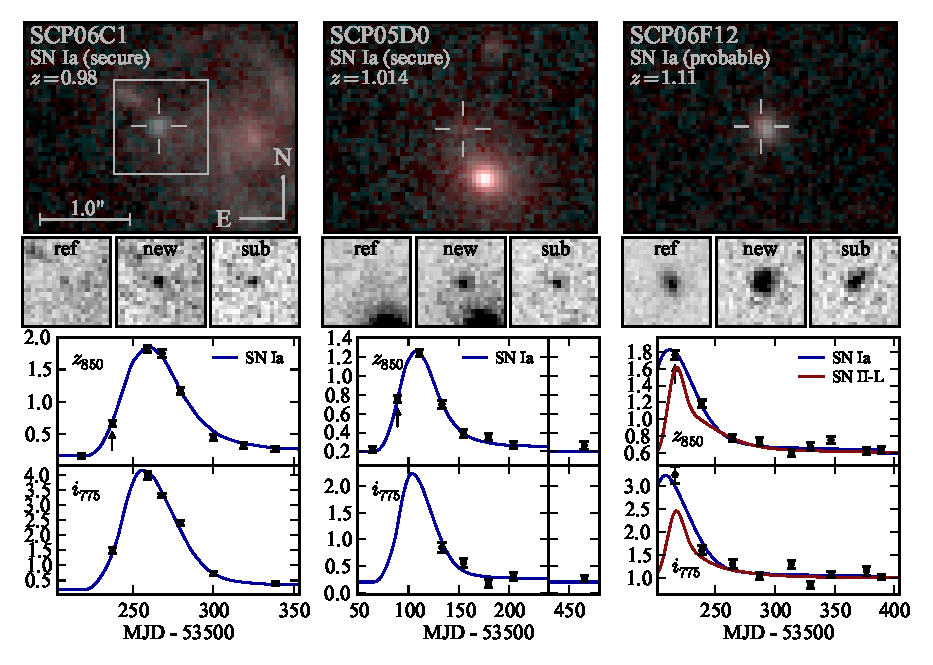
\includegraphics[width=\textwidth]{figures/cands/sn1.eps}
\caption[Images and light curves of candidates classified as
  supernovae.]{Images and light curves of the 29 candidates classified
  as supernovae. For each candidate, the \emph{top panel} shows the
  two-color stacked image ($i_{775}$ and $z_{850}$) of the supernova
  host galaxy, with the SN position indicated. The \emph{three smaller
    panels} below the stacked image show the reference, new, and
  subtracted images for the discovery visit. The \emph{bottom panel}
  shows the light curve at the SN position (including host galaxy
  light) in the $z_{850}$ ({\it top}) and $i_{775}$ ({\it bottom})
  bands. The y axes have units of counts per second in a $3$~pixel
  radius aperture. The effective zeropoints are 23.94 and 25.02 for
  $z_{850}$ and $i_{775}$, respectively. The discovery visit is
  indicated with an arrow in the $z_{850}$ plot. The best-fit SN~Ia
  template is shown in blue. For cases where the type is SN~Ia based
  on spectroscopic confirmation or host galaxy environment, only the
  best-fit SN~Ia template is shown, to demonstrate the consistency of
  the light curve with the designation. For cases where the type is
  based only on the light curve fit, the best-fit core collapse SN
  template is shown in red.  Note that the photometry used here is
  simple aperture photometry with fixed aperture corrections. For
  SN~Ia cosmology we use color-dependent aperture corrections, as
  described in \citet{suzuki11a}. [\emph{continued on next 5 pages.}]
\label{fig:sn}}
\end{figure}

\begin{figure}[p]
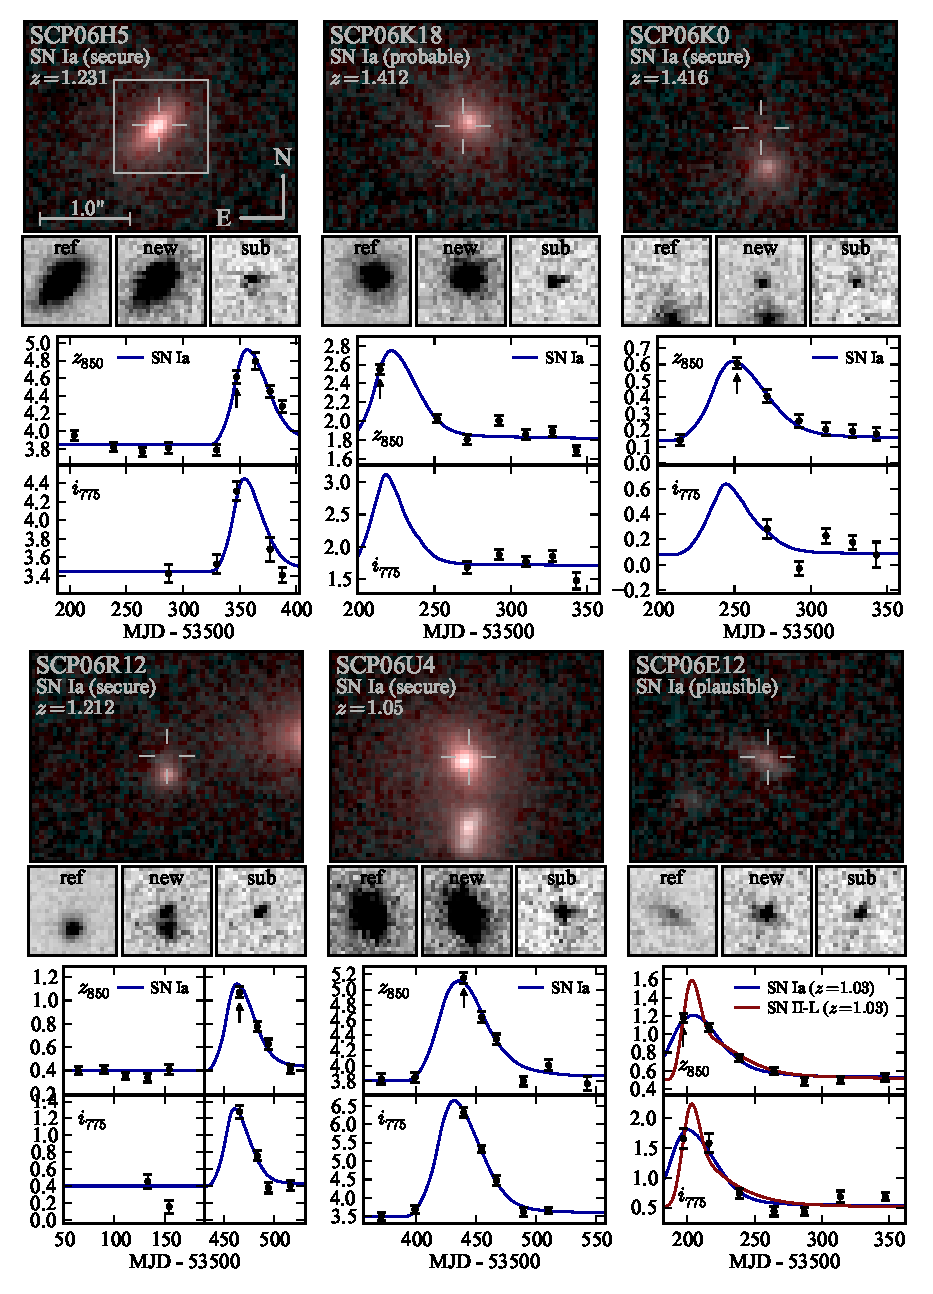
\includegraphics[width=\textwidth]{figures/cands/sn2.eps}
\end{figure}

\begin{figure}[p]
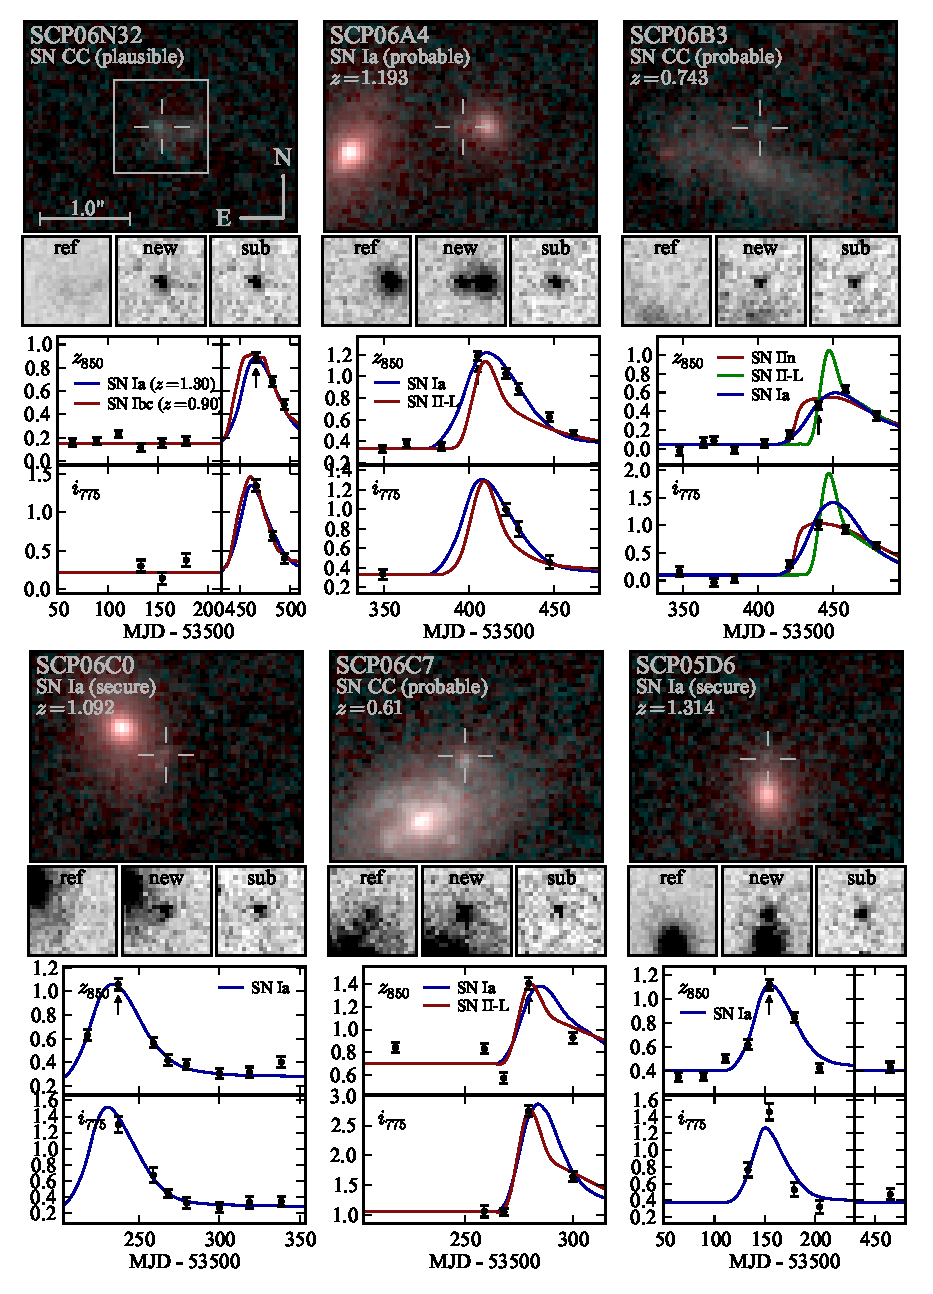
\includegraphics[width=\textwidth]{figures/cands/sn3.eps}
\end{figure}

\begin{figure}[p]
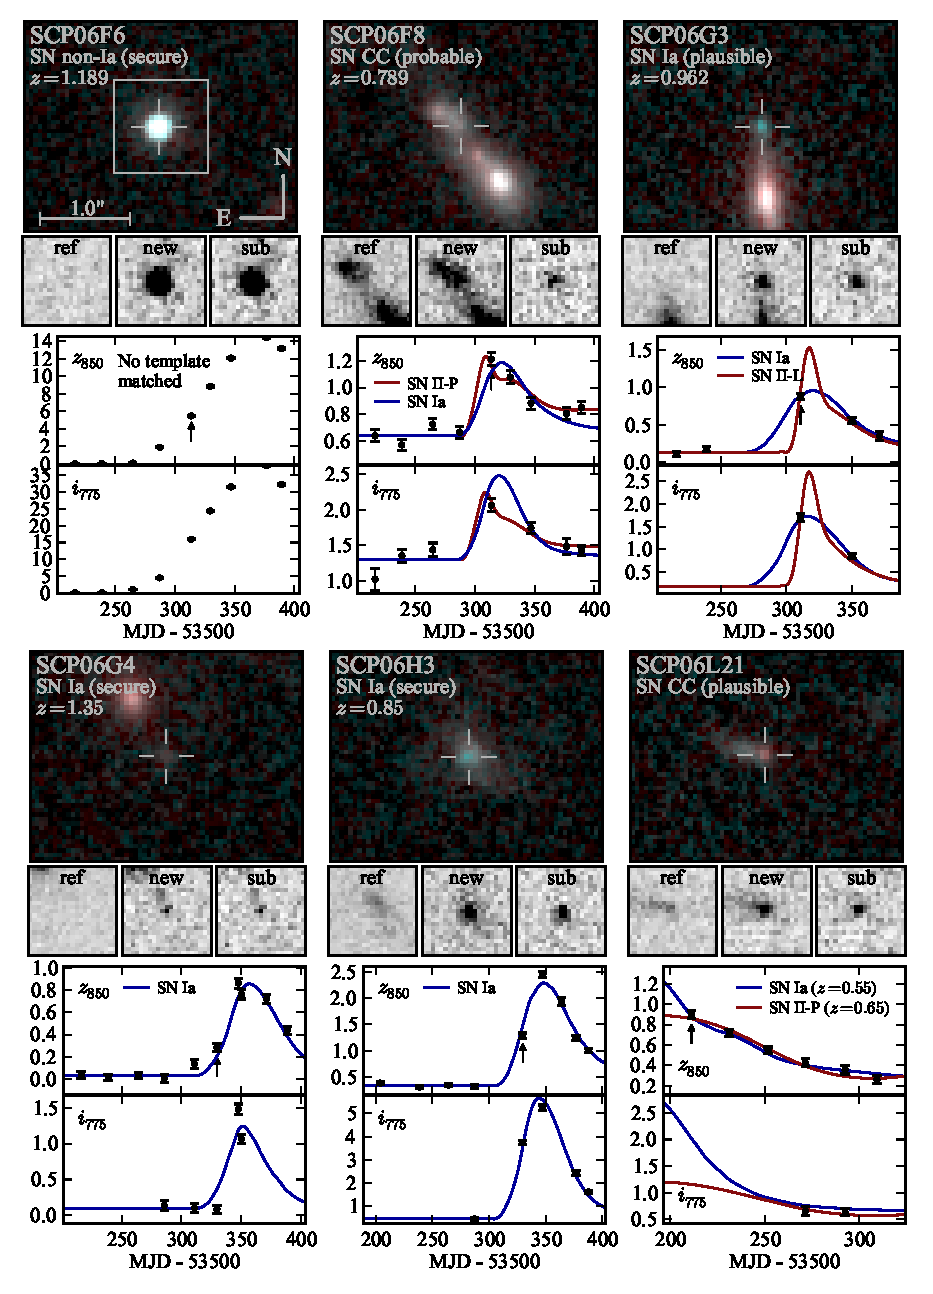
\includegraphics[width=\textwidth]{figures/cands/sn4.eps}
\end{figure}

\begin{figure}[p]
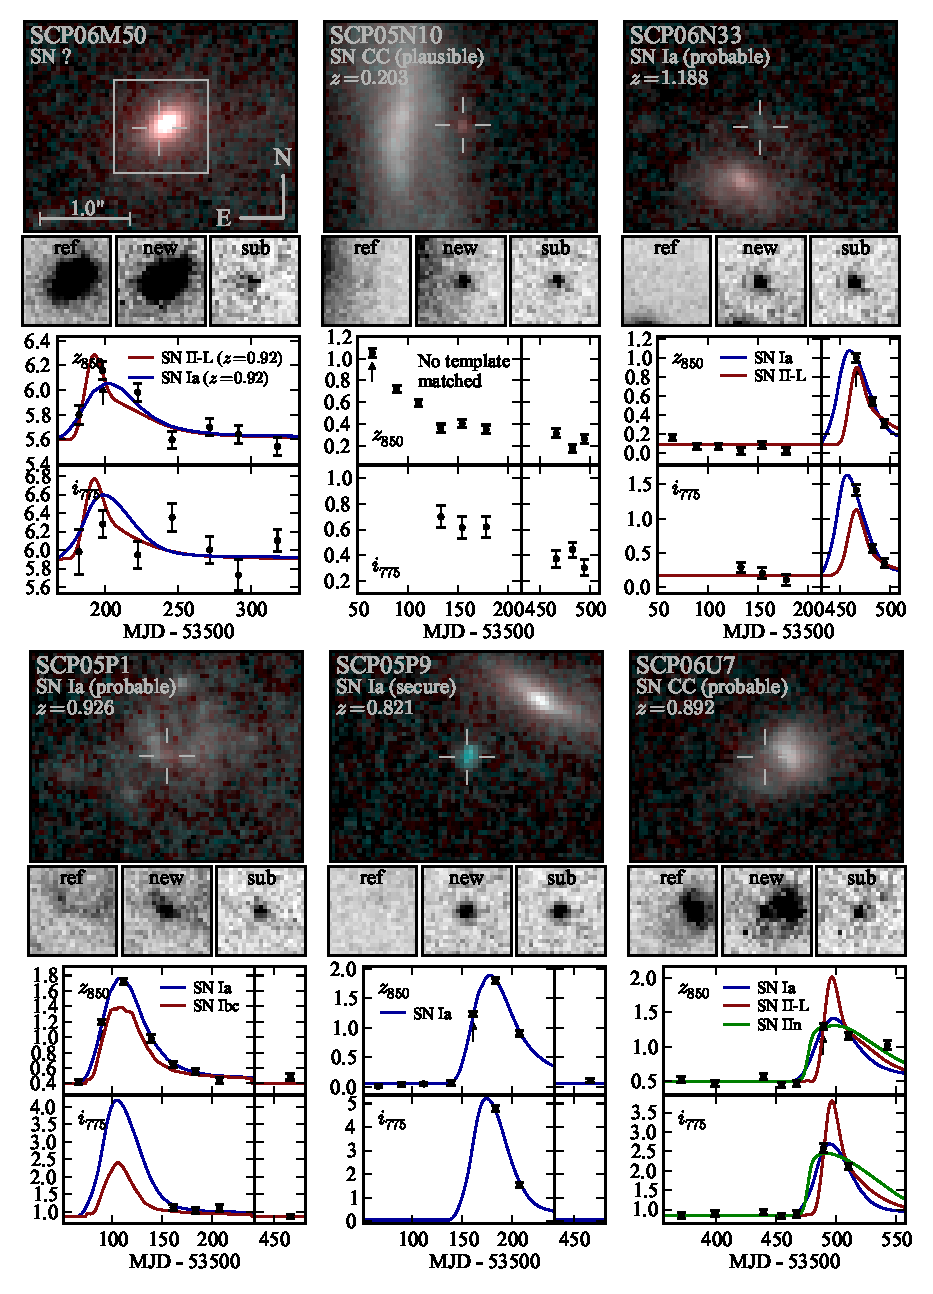
\includegraphics[width=\textwidth]{figures/cands/sn5.eps}
\end{figure}

\begin{figure}[t]
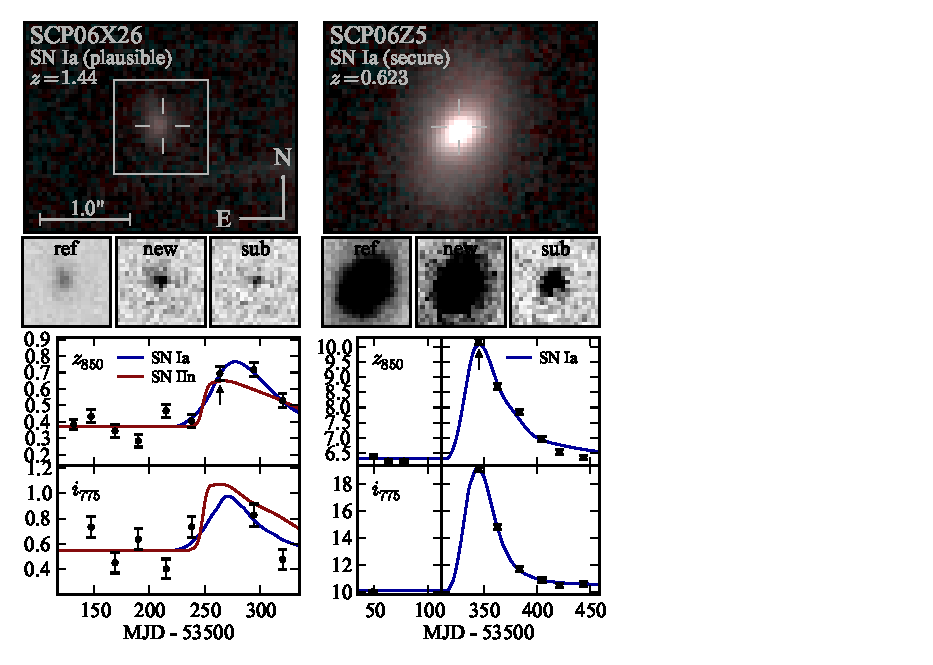
\includegraphics[width=\textwidth]{figures/cands/sn6.eps}
\end{figure}

%%%%%%%%%%%%%%%%%%%%%%%%%%%%%%%%%%%%%%%%%%%%%%%%%%%%%%%%%%%%%%%%%%%%%%%%
% end of SN candidates figures                                         %
%%%%%%%%%%%%%%%%%%%%%%%%%%%%%%%%%%%%%%%%%%%%%%%%%%%%%%%%%%%%%%%%%%%%%%%%


\begin{figure}[t]
\begin{center}
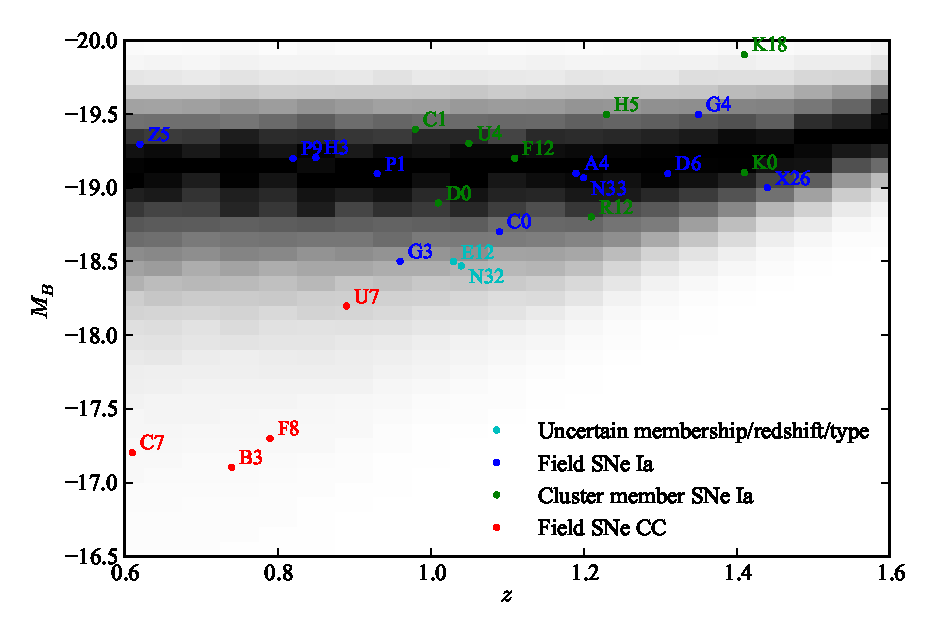
\includegraphics[width=\textwidth]{figures/cands/absmag_vs_z_field.eps}
\end{center}
\caption[Magnitude and redshift distribution of SN
  candidates]{Distribution of SNe in absolute magnitude and redshift,
  based on rough light curve fits. The shading represents the expected
  magnitude distribution of field SNe~Ia (similar for cluster SNe~Ia)
  in the survey in each redshift bin of $\Delta z = 0.05$, based on
  the simulations in \S\ref{sec:fieldrate_ct}. The candidates
  designated as core-collapse are all significantly dimmer than
  expected for SNe~Ia, while the distribution of SN~Ia candidates
  follows the expected distribution closely. Note that the light curve
  of SN SCP06K18 is very poorly constrained: $M_B \gtrsim -19.5$ is
  also consistent with the light curve data.\label{fig:absmag_vs_z}}
\end{figure}
